%========================================================================================%
%					NOTE
%========================================================================================%
% Probably this theme will not compile with standard pdftolatex compiler due to lack of some 
% fonts used in the theme. It is recommended to compile with XeLaTex instead.

% !TEX program = xelatex

%========================================================================================%
%					DOCUMENT SETUP
%========================================================================================%
\documentclass{beamer} 
\usetheme[progressbar=frametitle]{metropolis}

\usepackage{textpos}

\usepackage{amsmath}

\usepackage{mathrsfs}


%For making diagrams and drawing
\usepackage{tikz}
\usetikzlibrary{shapes,arrows, fit, positioning}

%For appendix
\usepackage{appendixnumberbeamer}


\usepackage[export]{adjustbox}

%Some additional graphcs tools
\usepackage{graphicx}
%\usepackage{datatool}
%\usepackage{animate}
\graphicspath{{../figs/}}

% For someone using the pgfplot tools
%\usepackage{pgfplots}
%\usepgfplotslibrary{dateplot, groupplots}
%\pgfplotsset{compat=1.14}
%\usepgfplotslibrary{fillbetween}

%Remove words break, wrap instead
\usepackage[none]{hyphenat}

\usepackage{minted}

%for custom date
\usepackage[english]{babel}
\usepackage[nodayofweek,level]{datetime}

\usepackage{xspace}
\newcommand{\themename}{\textbf{\textsc{metropolis}}\xspace}

\renewcommand*{\arraystretch}{1.2}

\usefonttheme[onlymath]{serif}




%===================================================================================%
%				FRONT PAGE
%===================================================================================%
\titlegraphic{%
\hfill%

\includegraphics[height=1.5cm, valign=c]{logos/ccfd3.png}%
\hspace{15pt}%

\includegraphics[height=1.5cm, valign=c]{logos/symbol-PL.pdf}%
}

\title{Introduction to concurrency in modern C++}
\date{\vspace{5pt}\formatdate{16}{1}{2023}}
\author{Jakub Gałecki}

%===================================================================================%
%				THEME COLORS
%===================================================================================%
% specify main colors which are being used by the theme
\definecolor{bordercolor}{HTML}{002699}
\definecolor{fillcolor}{HTML}{002699}

% fix theme black color which affects tikz plots
\definecolor{black}{RGB}{0,0,0}




%===================================================================================%
%				ACTUAL DOCUMENT CONTENT
%===================================================================================%

\begin{document}

\maketitle

%force to add logos to the each frame title
\addtobeamertemplate{frametitle}{}{%
\begin{textblock*}{100mm}(.9\textwidth,-0.9cm)

\includegraphics[height=0.8cm, valign=c]{logos/ccfd3_white.png}\hspace{10pt}
\includegraphics[height=0.78cm, valign=c]{logos/symbol-PL-white.pdf}
\end{textblock*}}

\begin{frame}{Disclaimer}
This will be a firehose talk.
It's meant to serve as a broad overview, not an exhaustive reference.
\begin{center}
\vspace{.1cm}

\includegraphics[width=\linewidth]{firehose.jpg}
\end{center}
\end{frame}

\begin{frame}[standout]
Introduction
\end{frame}

\begin{frame}{One CPU, multiple cores}
\begin{center}
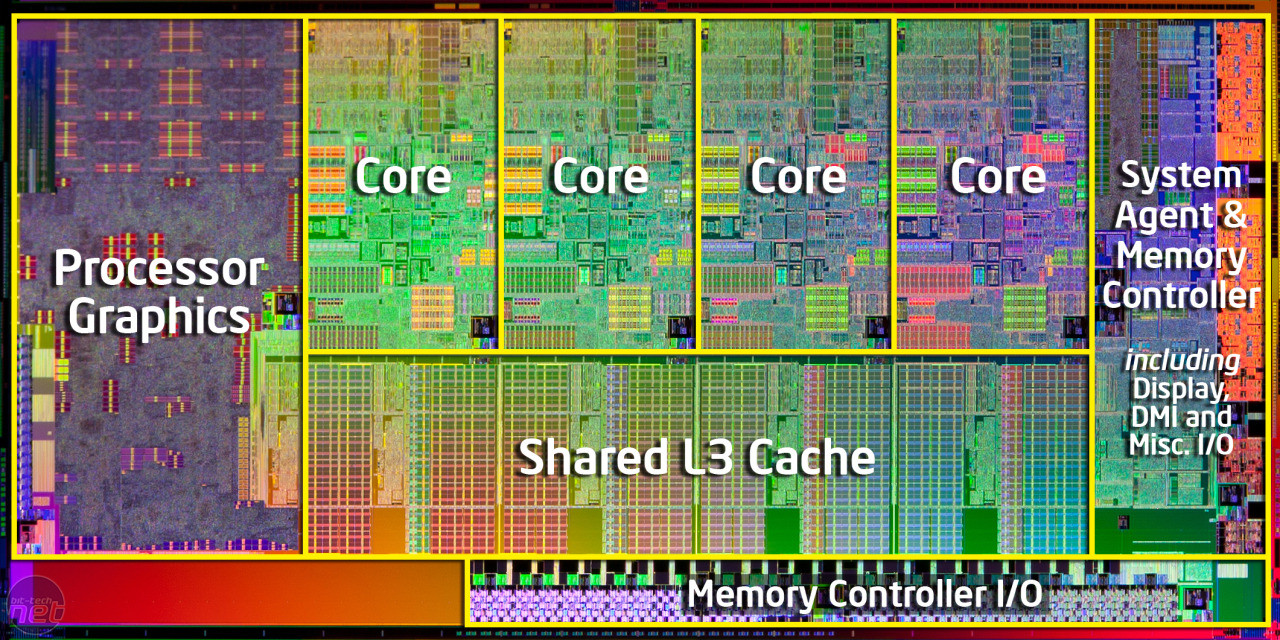
\includegraphics[width=\linewidth]{cpu_die.jpg}
\end{center}
\end{frame}

\begin{frame}{Process vs. thread}
\begin{center}
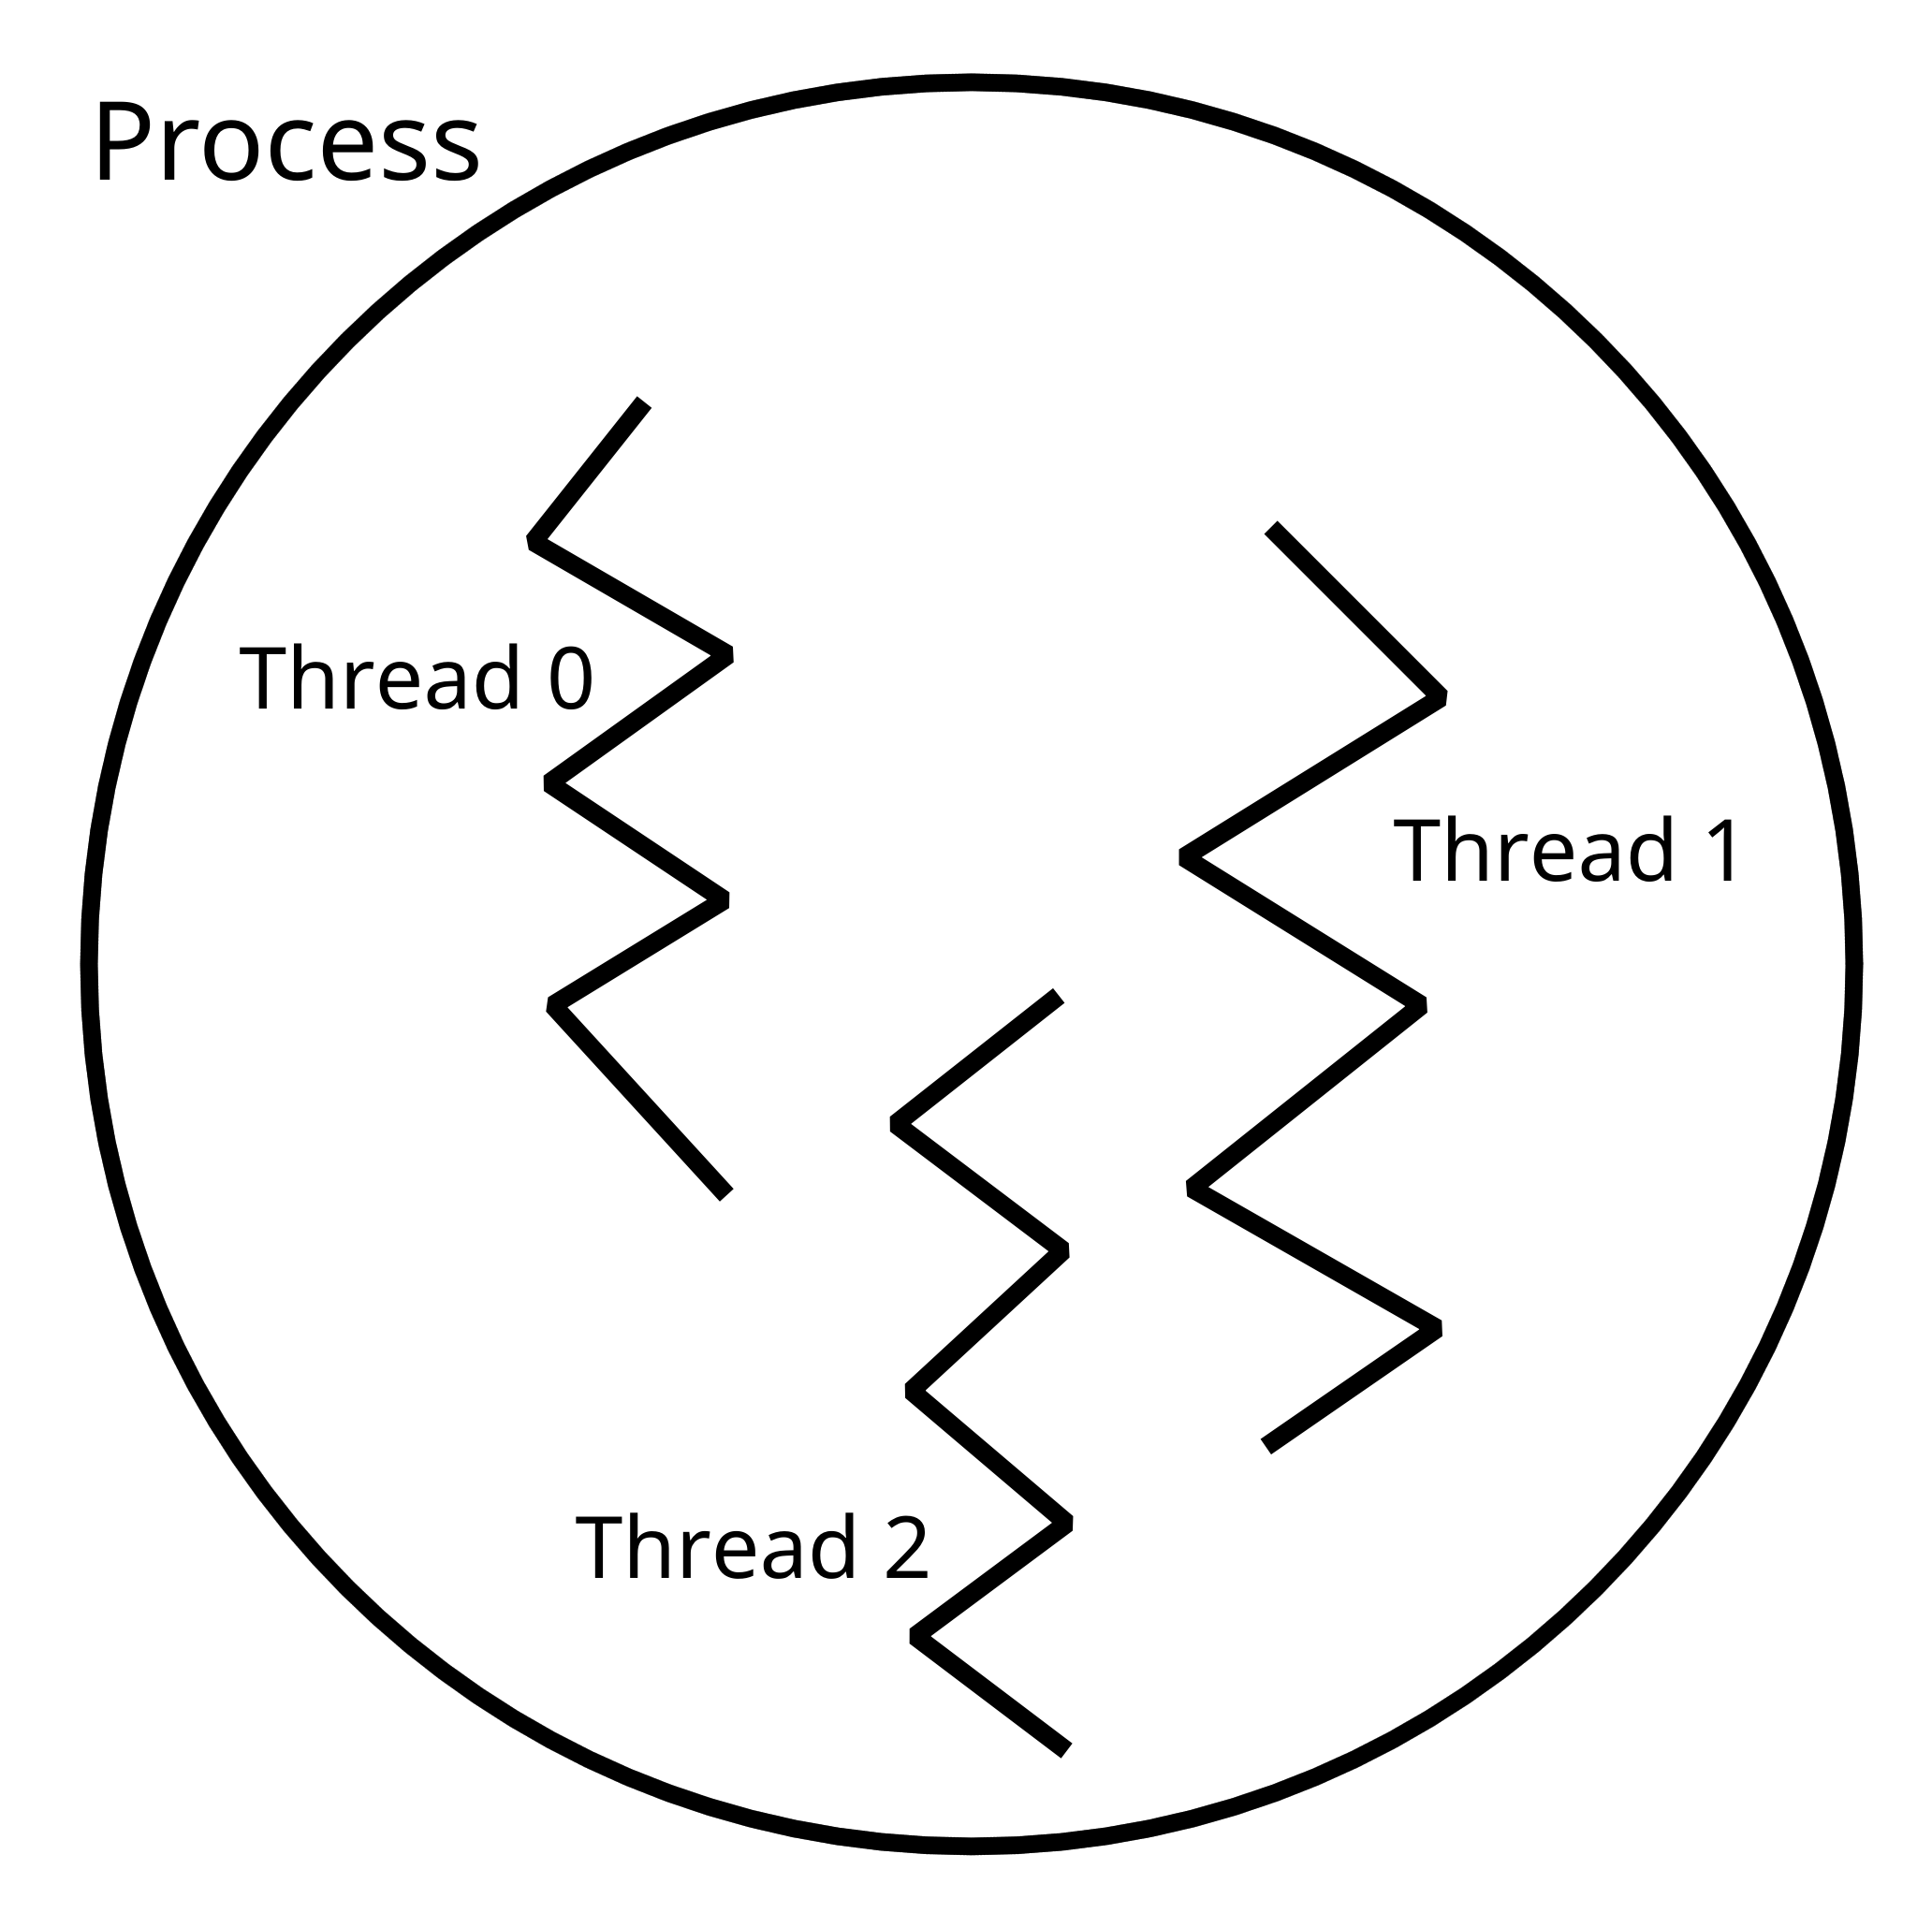
\includegraphics[width=.65\linewidth]{proc_thread.png}
\end{center}
\end{frame}

\begin{frame}{Process vs. thread}
\begin{columns}
\begin{column}{0.5\textwidth}
\textbf{Process} \\
\begin{itemize}
\item Has its own address space
\item Walled off from other processes
\item consists of at least one thread
\item When you launch an application, you launch a process (and its main thread)
\end{itemize}
\end{column}
\begin{column}{0.5\textwidth}
\textbf{Thread} \\
\begin{itemize}
\item Smallest logical unit of execution, single stream of instructions
\item Belongs to a process
\item Stateful
\item \textbf{Shares the address space of the process with other threads}
\end{itemize}
\end{column}
\end{columns}

\vspace{.3cm}
The OS is aware of and manages both processes and threads
\end{frame}

\begin{frame}{Example}
\tiny
\begin{columns}
\begin{column}{0.5\textwidth}
\inputminted{cpp}{../code/examples/example01a.cpp}

\vspace{.25cm}
\hrulefill

\texttt{Hello from thread 1}

\texttt{Hello from thread 2}

\vspace{.25cm}
\hrulefill

\texttt{Hello from thread 2}

\texttt{Hello from thread 1}

\vspace{.25cm}
\hrulefill

\texttt{Hello from thread Hello from thread 12}
\end{column}
\begin{column}{0.5\textwidth}
\inputminted{cpp}{../code/examples/example01b.cpp}

\vspace{.25cm}
\hrulefill

\texttt{139765188224576}

\texttt{139765179831872}
\end{column}
\end{columns}
\end{frame}

\begin{frame}{Example}
\scriptsize
\inputminted{cpp}{../code/examples/example02.cpp}

\vspace{.25cm}
\hrulefill

\texttt{1004817}
\end{frame}

\begin{frame}{Races}
\metroset{block=fill}
\begin{block}{Data race}
A data race (race condition) occurs iff multiple threads access an object and at least one of them modifies it
\end{block}

Thread synchronization is critical

We need to structure our multithreaded programs to
\begin{itemize}
\item \textbf{avoid data races}
\item ensure correctness
\item have good performance
\end{itemize}
\end{frame}

\begin{frame}{Summary of concurrent facilities in the STL}
\begin{itemize}
\item \texttt{jthread} - manage a thread (start, join, request stop)
\item \texttt{mutex} - mutual exlusion lock
\item \texttt{semaphore} - constrains access to a resource
\item \texttt{barrier}/\texttt{latch} - synchronize a team of threads
\item \texttt{promise} + \texttt{future} - synchronize work between a producer and consumer
\item \texttt{condition\_variable} - wait until a condition is met
\item \texttt{atomic} - fine-grained atomic operations
\end{itemize}
\end{frame}

\begin{frame}{Amdahl's law}
Given work which has available parallelism $p$ and $n$ workers, the highest speedup we can achieve is
\begin{equation*}
S(p,n)=\frac{1}{\left(1 - p\right) + \frac{p}{n}}
\end{equation*}

\begin{center}
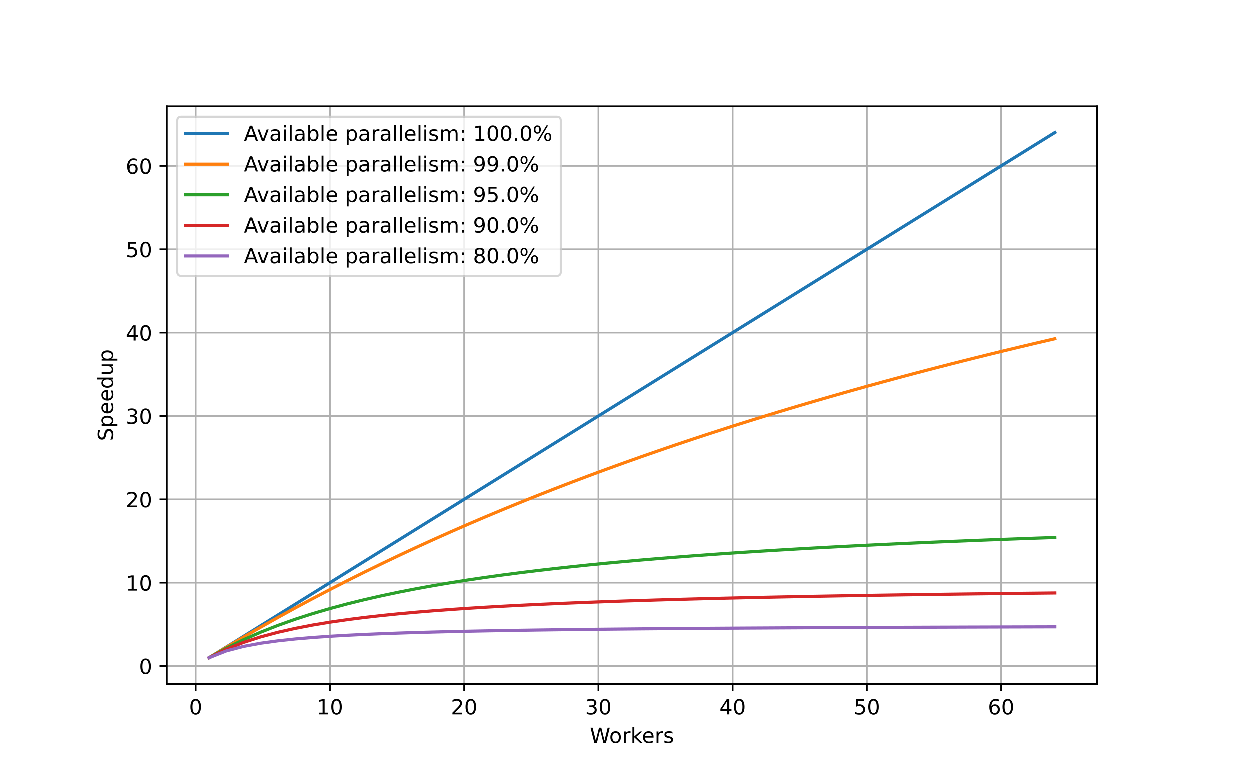
\includegraphics[width=.8\textwidth, trim = {1cm, .25cm, 1cm, 1.25cm}, clip]{amdahl.eps}
\end{center}
\end{frame}

\begin{frame}{Multithreading}
\begin{center}
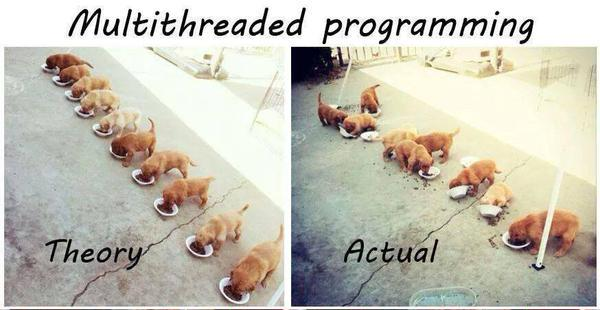
\includegraphics[width=\linewidth]{concurrency.jpeg}
\end{center}
\end{frame}

\begin{frame}{Universal scalability law}
\begin{center}
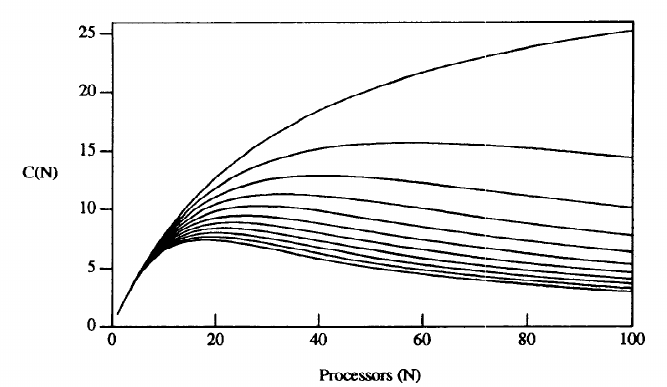
\includegraphics[width=\textwidth]{usl.png}
\end{center}

\tiny
N. J. Gunther, "A Simple Capacity Model of Massively Parallel Transaction Systems," CMG National Conference, 1993
\end{frame}

\begin{frame}[standout]
Case study: task queue
\end{frame}

\begin{frame}{Motivating example}
Hashing a vector of strings
\begin{itemize}
\item String comes in
\item Magic happens
\item 64 bit unsigned integer comes out
\end{itemize}

Let's take a look at the serial code...

This seems easy to parallelize. What could possibly go wrong?
\end{frame}

\begin{frame}{Task Queue}
Task = Callable + Arguments

Task queue stores tasks and executes them in FIFO order on a thread pool

Use futures to query the completion of individual tasks

Performance!

What are some of the ways we could implement this?

\tiny\vfill
\url{https://youtu.be/zULU6Hhp42w}

\url{https://sean-parent.stlab.cc/presentations/2017-01-18-concurrency/2017-01-18-concurrency.pdf}
\end{frame}

\begin{frame}[standout]
The features
\end{frame}

\begin{frame}[fragile]{Variadic templates}
We can write templates with an unspecified number of parameters

Syntax: \texttt{template <typename ... T>}

The above can be instantiated with any number of types (including zero)

\texttt{T} is a parameter pack and must be expanded whenever used

\scriptsize
\vspace{.5cm}
\begin{minted}{cpp}
template <typename F, typename ...Args>
auto invoke(F f, Args... args) {
  return f(args...);
}
\end{minted}
\end{frame}

\begin{frame}[fragile]{Universal reference, Perfect forwarding}
When writing a function taking arguments by lvalue or rvalue reference, you need to write 2 functions

When writing a function \textit{template} taking arguments by reference, we can avoid this by using universal references

Universal reference: \texttt{T\&\&}, where \texttt{T} is a function parameter

Use \texttt{std::forward} to pass as lvalue (do nothing) or rvalue (move)

\scriptsize
\vspace{.5cm}
\begin{minted}{cpp}
template <typename F, typename ...Args>
auto invoke(F&& f, Args&&... args) {
  return f(std::forward<Args>(args)...);
}
\end{minted}
\end{frame}

\begin{frame}[fragile]{\texttt{std::[move\_only\_]function}}
Type-erased function wrapper

Template syntax: \texttt{std::function<R(Args...)>}

Wraps arbitrary function object which takes arguments of types \texttt{Args...} and returns \texttt{R}

\scriptsize
\vspace{.5cm}
\begin{minted}{cpp}
using fun_t = std::function<double(double)>;

fun_t times5{[a = 5.](double arg) {
  return a * arg;
}};

double foo(double) { /* ... */ }
fun_t wrapped_foo{foo};
\end{minted}
\end{frame}

\begin{frame}[fragile]{\texttt{std::bind[\_front/\_back]}}
Packages a callable along with some number of arguments

``\texttt{std::function} with some arguments already included''

\scriptsize
\vspace{.5cm}
\begin{minted}{cpp}
double minus(double a, double b) { return a - b; }
// ...
const auto ten_minus = std::bind_front(minus, 10);
std::cout << ten_minus(3) << '\n';
\end{minted}

\vspace{.25cm}
\hrulefill

\texttt{7}
\end{frame}

\begin{frame}{\texttt{std::mutex}}
In concurrent programming, we often need to execute some sequence of operations while ensuring that some shared state is not accessed from another thread

Such a sequence of operations is called a critical section

We can use a mutex to protect a critical section

To exclude other threads we \textbf{lock} the mutex, once we're done we \textbf{unlock} it

Always use a RAII wrapper: e.g. \texttt{std::lock\_guard}, \texttt{std::unique\_lock}, \texttt{std::scope\_guard}
\end{frame}

\begin{frame}[fragile]{\texttt{std::mutex}}
\scriptsize
\inputminted{cpp}{../code/examples/example03.cpp}

\vspace{.25cm}
\hrulefill

\texttt{2}
\end{frame}

\begin{frame}{\texttt{std::future}}
Used to communicate work done asynchronously

\texttt{get} waits for completion and returns the result

\scriptsize
\vspace{.25cm}
\inputminted{cpp}{../code/examples/example04.cpp}

\vspace{.25cm}
\hrulefill

\texttt{42}
\end{frame}

\begin{frame}{\texttt{std::condition\_variable[\_any]}}
Synchronization primitive which allows a thread to sleep until a condition is satisfied

Sleeping threads don't take up CPU time

\texttt{wait} to go to sleep

\texttt{notify\_one} or \texttt{notify\_all} to wake up threads waiting on a condition variable
\end{frame}


\begin{frame}[fragile]{\texttt{std::condition\_variable[\_any]}}
\tiny
\inputminted{cpp}{../code/examples/example05.cpp}
\end{frame}

\begin{frame}[standout]
Results \& conclusions
\end{frame}

\begin{frame}{Results summary, 4x nehalem}
\begin{center}
\hspace{-0.65cm}
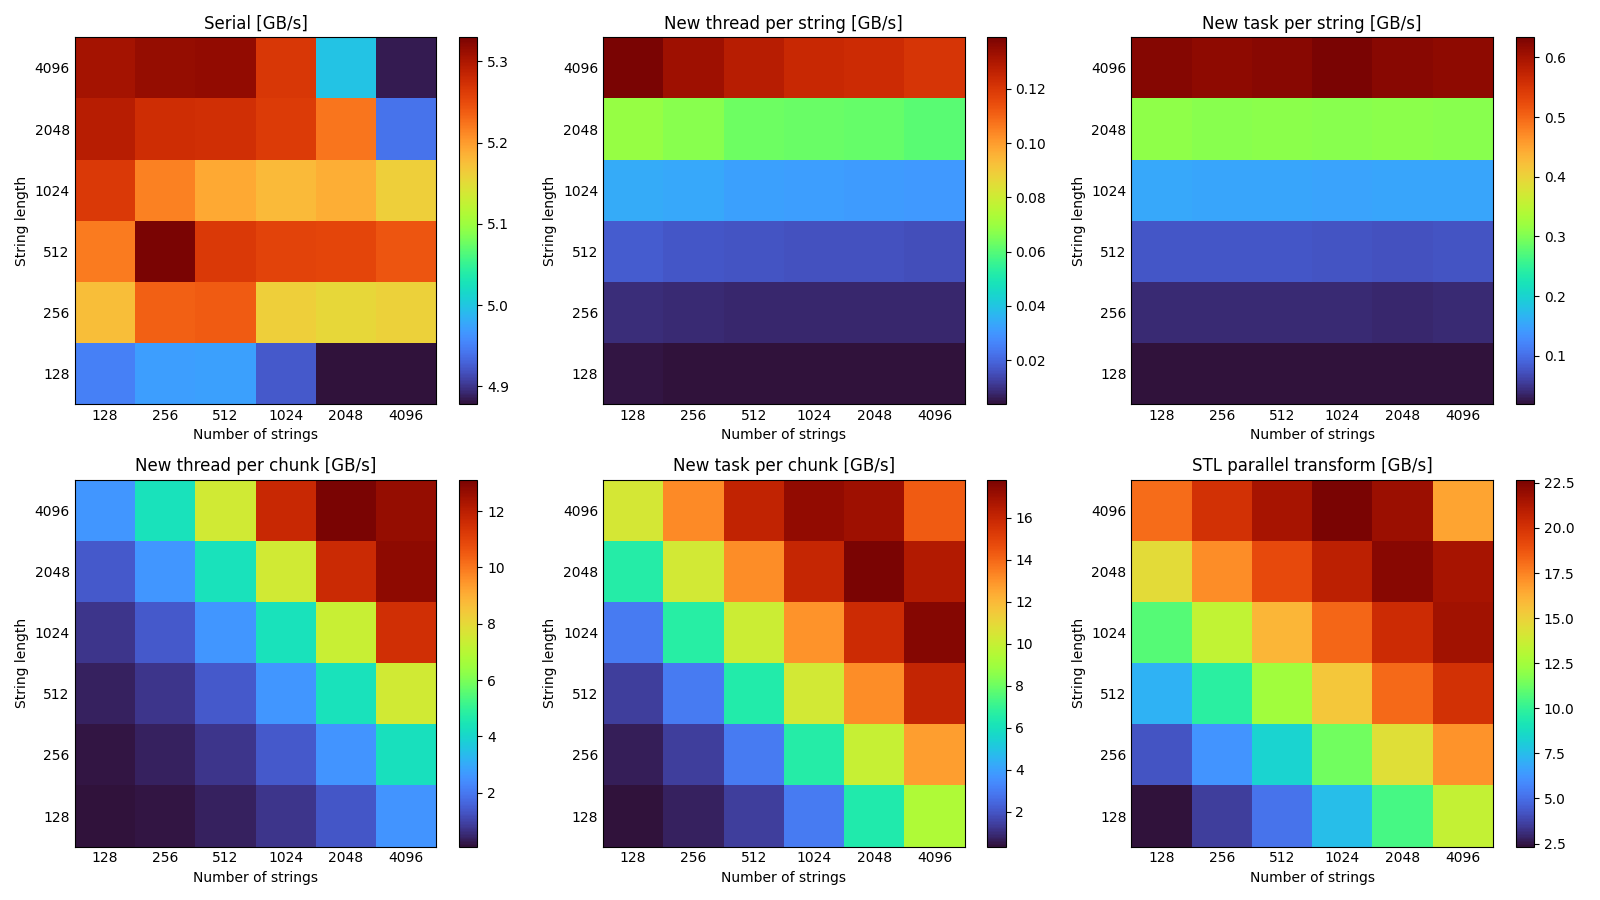
\includegraphics[width=1.05\textwidth, trim = {.25cm, 0cm, .6cm, 0cm}, clip]{nehalem_4cores_results.png}
\end{center}
\end{frame}

\begin{frame}{Results summary, 8x skylake}
\begin{center}
\hspace{-0.65cm}
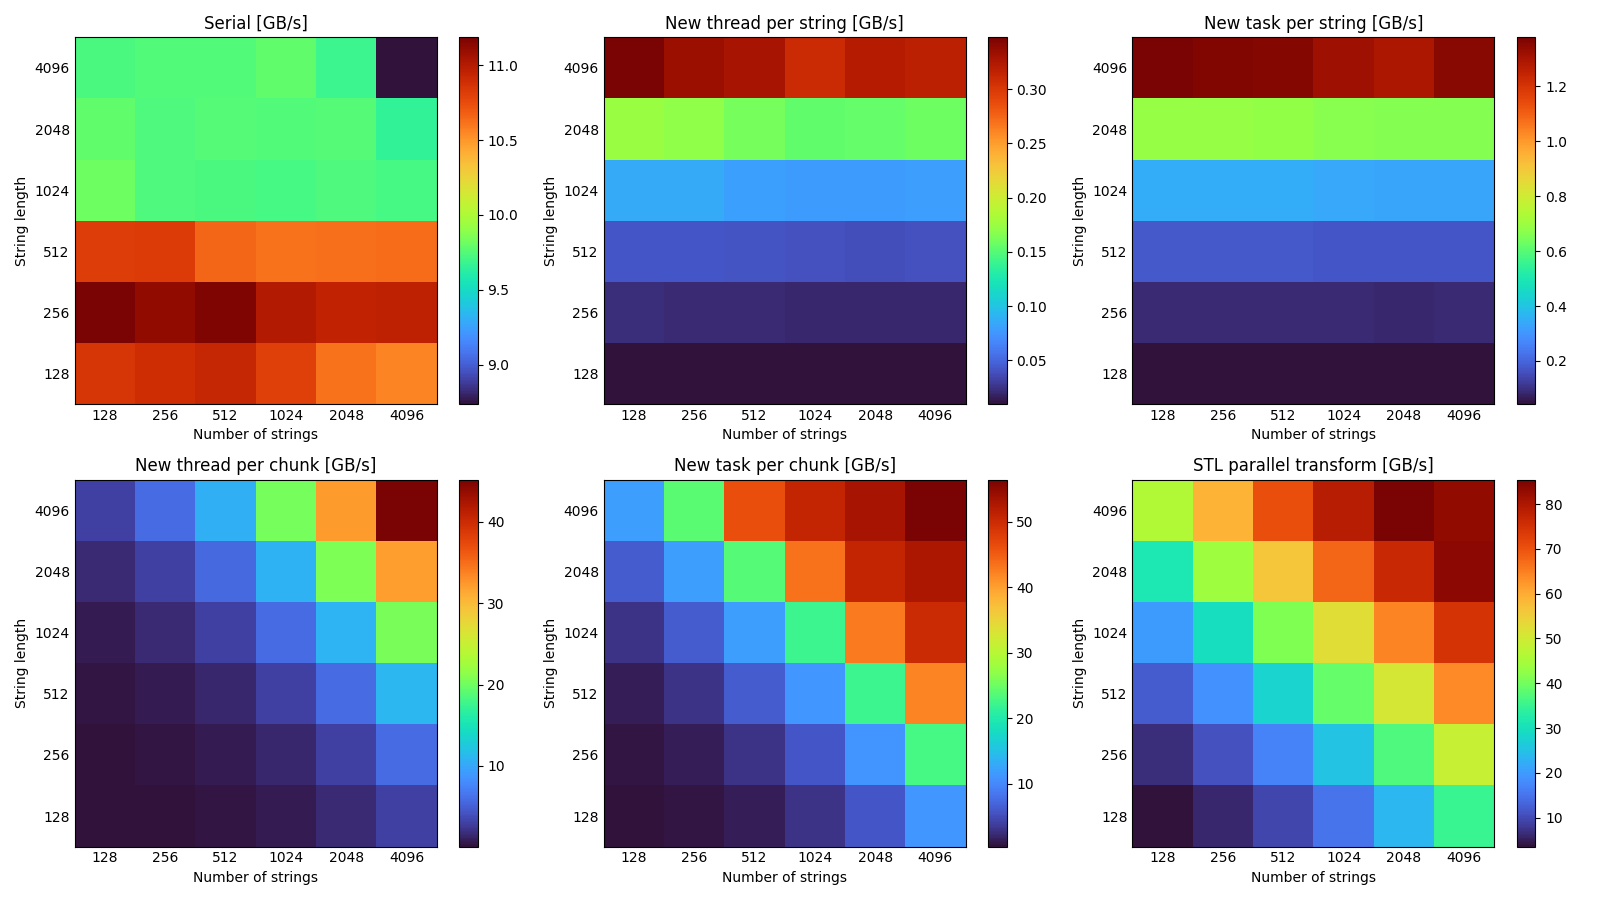
\includegraphics[width=1.05\textwidth, trim = {.25cm, 0cm, .6cm, 0cm}, clip]{skylake_8cores_results.png}
\end{center}
\end{frame}

\begin{frame}{Summary}
\begin{itemize}
\setlength\itemsep{.5em}
\item Multithreading is \underline{hard}
\item Manually managing threads is usually a bad idea
\item The STL has some very useful concurrency primitives
\item Generic programming is a great tool, which yields powerful abstractions
\item Balance your load
\end{itemize}
\end{frame}

\begin{frame}{Key takeaways}
\Large
\begin{itemize}
\setlength\itemsep{1em}
\item[\rightarrow] Don't assume anything about performance that you haven't measured
\item[\rightarrow] Rely on established, optimized libraries
\item[\rightarrow] C++ is old, but it's evolving rapidly, and you just can't beat the performance!
\end{itemize}
\end{frame}

\appendix
\begin{frame}{Thanks for listening}
\Large
If you'd like to learn more about optimizing software performance (among other things), sign up for our ``Intro to HPC'' course next semester!

\vfill
Questions?
\end{frame}
\end{document}
